%!TEX root = pag0.tex

\chapter{Modello della camera}
\label{chapter2}


La camera utilizzata è una camera monoculare posta sul end-effector del braccio robotico. Questo tipo di telecamera ha un ingombro minimo, ma si perde la percenzione della distanza. Per ricostruire queste informazioni occorre utilizzare la \emph{stereo visione}\footnote{Stima della profondità tramite l'utilizzo di due immagini della stessa scena prese da angolazioni differenti} utilizzando la \emph{geometria epipolare} \footnote{Essa descrive le relazioni e i vincoli geometrici che legano due immagini 2D della stessa scena 3D catturata da due fotocamere con posizione e orientamento distinto}. 
La camera utilizzata nel progetto è la camera monoculare della Playstation 3 mostrata in Fig ~\ref{fig:camera} di produzione della Sony con una risoluzione di 640X480 pixel. 
\begin{figure}[H]
   \centering
   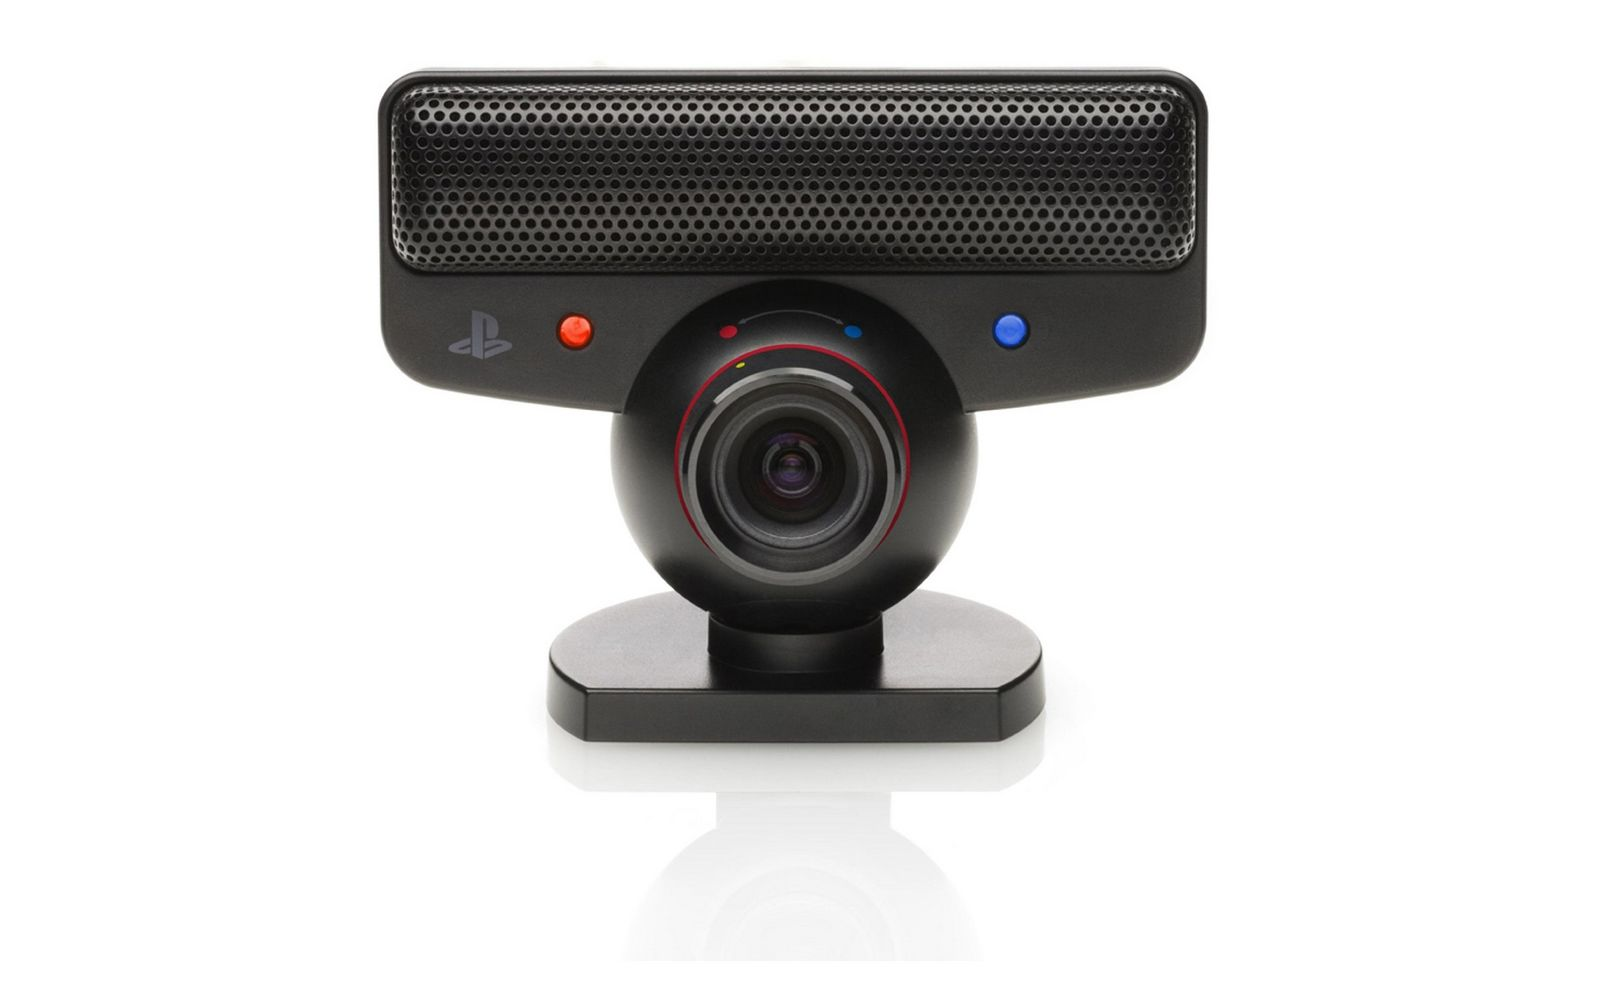
\includegraphics[width=.7\columnwidth]{camera.jpg}
   \caption{Camera utilizzata nel progetto}
   \label{fig:camera} 
\end{figure}


\newpage 
\subsection{Modello pinhole}
La geometria di tale modello prevede che i raggi luminosi provenienti dal mondo che passano attraverso un foro di dimensione infinitesima, vadano a formare l'immagine su un piano disposto dietro il foro, chiamato \emph{piano immagine}. In termini matematici consideriamo un punto nel mondo con cordinate $X_c = [X_c, Y_c, Z_c]^T $ il cui sistema di riferimento $O$ è centrato nel foro. Questo sistema di riferimento prende il nome di \emph{centro ottico}. L'asse $z$ è l'asse ottico, ed è la retta perpendicolare al piano dell'immagine passante per il centro ottico. Il raggio luminoso che segue l'asse ottico è chiamato \emph{raggio principale}. La distanza fra il piano immagine e il centro ottico è la \emph{lunghezza focale} $f$. La figura ~\ref{fig:pinhole} mostra lo schema di queste definizioni.
\begin{figure}[H]
   \centering
   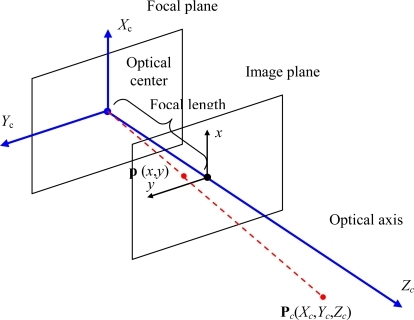
\includegraphics[width=.7\columnwidth]{pinhole.png}
   \caption{Modello schematico del modello pinhole}
   \label{fig:pinhole} 
\end{figure}
Con queste definizioni possiamo chiamare \emph{parametri instrinseci} tutti quei parametri necessari a collegare le coordinate di un pixel dell'immagine con le coordinate corrispondenti nel sistema di riferimento della camera. In altre parole sono i parametri necessari a specificare le caratteristiche ottiche, geometriche e digitali della camera. Tali parametri sono:
\begin{itemize}
\item la lunghezza focale
\item le coordinate in pixel del centro dell'immagine
\item la distorsione geometrica 
\item la dimensione dei pixel
\end{itemize}
I \emph{parametri estrinseci} sono tutti quei parametri che definiscono la posizione ed orientazione del sistema di riferimento della camera rispetto al riferimento mondo. Sono un insieme di parametri geometrici che identificano univocamente le trasformazioni tra il sistema di riferimento della camera e quello mondo, supposto noto. Tali parametri sono:
\begin{itemize}
\item vettore di traslazione
\item matrice di rotazione 3x3 ortogonale
\end{itemize}
Il punto sul piano immagine $x = [x_i,y_i]^T$ corrispondente a $X_c$ è definito come in figura ~\ref{fig:images_point} 
\begin{figure}[H]
   \centering
   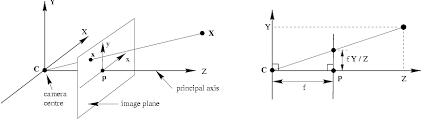
\includegraphics[width=1\columnwidth]{images_point.png} 
   \caption{Punti nel piano immagine}
   \label{fig:images_point} 
\end{figure}
\begin{equation}
\begin{cases}
x_i = f_x * \frac{X_c}{Z_c}	+ c_x\\	
y_i = f_y* \frac{Y_c}{Z_c} + c_y
 \end{cases}
\label{eq:punto_immagine}
\end{equation}
Utilizzando il modello pinhole, il punto $X_c$ proiettato nel piano immagine è esprimibile come:
\begin{equation}
 s* \begin{bmatrix}
    x  \\
    y \\
    1
  \end{bmatrix} = \begin{bmatrix}
    f_x & 0&c_x  \\
    0&f_y&c_y \\
    0&0&1
  \end{bmatrix} * \begin{bmatrix}
  r_{11} & r_{12} & r_{13} & t_1 \\
  r_{21} & r_{22} & r_{23} & t_2	\\
  r_{31} & r_{32} & r_{33} & t_{3}
  \end{bmatrix} *\begin{bmatrix}
    X_c  \\
    Y_c \\
    Z_c \\
  \end{bmatrix}
\label{eq:punto omogeneo}
\end{equation}
Dove $c_x$ e $c_y$ sono i centri ottici espressi in pixel e $A$ è la matrice dei parametri intrinseci, il fattore $s$ che moltiplica il vettore dei punti nel piano immagine è detto \emph{fattore di scala}. La matrice di roto-traslazione è chiamata matrice dei parametri estrinseci, ed è usata per descrivere il moto della camera attorno ad una scena statica. Nella figura ~\ref{fig:modello_pin} si può vedere uno schema del modello pinhole con la descrizione dei parametri intrinseci ed estrinseci.
\begin{figure}[H]
   \centering
   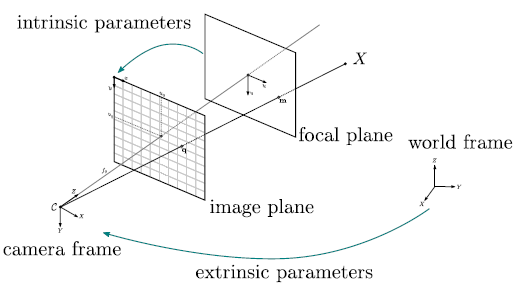
\includegraphics[width=0.7\columnwidth]{pinholeCamera.png} 
   \caption{Schema del modello pinhole con parametri estrinseci ed intrinseci}
   \label{fig:modello_pin} 
\end{figure}



